%%%%%%%%%%%%%%%%%%%%%%%%%%%%%%%%%%%%%%%%%%%%%%%%%%%%%%%%%%%%%%%%%%%%%%%%%%%%%%%%
% File acl2015.tex
%
% Contact: car@ir.hit.edu.cn, gdzhou@suda.edu.cn
%
% Based on the style files for ACL-2014, which were, in turn,
% Based on the style files for ACL-2013, which were, in turn,
% Based on the style files for ACL-2012, which were, in turn,
% based on the style files for ACL-2011, which were, in turn, 
% based on the style files for ACL-2010, which were, in turn, 
% based on the style files for ACL-IJCNLP-2009, which were, in turn,
% based on the style files for EACL-2009 and IJCNLP-2008...

% Based on the style files for EACL 2006 by 
% e.agirre@ehu.es or Sergi.Balari@uab.es
% and that of ACL 08 by Joakim Nivre and Noah Smith

\documentclass[11pt]{article}

\usepackage{acl2015}
\usepackage[utf8]{inputenc}
\usepackage{times}
\usepackage{url}
\usepackage{latexsym}
\usepackage{color}
\usepackage{tikz}
\usepackage{pgfplots}
\usepackage{lipsum}
\usepackage{units}
\usepackage{amsmath}
\usepackage{relsize}
\usepackage{booktabs}
\usepackage{multirow}

%\setlength\titlebox{5cm}

\usetikzlibrary{arrows, backgrounds, decorations.markings, positioning, shapes}

\newcommand\TODO[1]{\textcolor{red}{[TODO #1]}}
\newcommand\FILL[1]{\textcolor{red}{\lipsum[#1]}}

%% tikz pictures %%%%%%%%%%%%%%%%%%%%%%%%%%%%%%%%%%%%%%%%%%%%%%%%%%%%%%%%%%%%%%%
\tikzstyle{arrow}=[
  decoration={markings, mark=at position 1 with {\arrow[scale=2.5]{>}}},
  postaction={decorate}
]

%-- database -------------------------------------------------------------------
% http://tex.stackexchange.com/questions/123854/display-database-instance-relationship-with-tikz
\tikzstyle{database}=[
  draw,
  color=black,
  align=center,
  minimum width=5.5em,
  minimum height=6.5em,
  cylinder,
  cylinder uses custom fill,
  cylinder body fill=White,
  cylinder end fill=White,
  shape border rotate=90,
  aspect=0.5
]
\newcommand\drawdatabase[1]{
  \begin{tikzpicture}
    \node[database] (db) {#1};
  \end{tikzpicture}
}

%-- document -------------------------------------------------------------------
% http://tex.stackexchange.com/questions/103688/folded-paper-shape-tikz
\makeatletter
\pgfdeclareshape{doc}{
  \inheritsavedanchors[from=rectangle] % this is nearly a rectangle
  \inheritanchorborder[from=rectangle]
  \inheritanchor[from=rectangle]{center}
  \inheritanchor[from=rectangle]{north}
  \inheritanchor[from=rectangle]{south}
  \inheritanchor[from=rectangle]{west}
  \inheritanchor[from=rectangle]{east}
  % ... and possibly more
  \backgroundpath{% this is new
    % store lower right in xa/ya and upper right in xb/yb
    \southwest \pgf@xa=\pgf@x \pgf@ya=\pgf@y
    \northeast \pgf@xb=\pgf@x \pgf@yb=\pgf@y
    % compute corner of ‘‘flipped page’’
    \pgf@xc=\pgf@xb \advance\pgf@xc by-10pt % this should be a parameter
    \pgf@yc=\pgf@yb \advance\pgf@yc by-10pt
    % construct main path
    \pgfpathmoveto{\pgfpoint{\pgf@xa}{\pgf@ya}}
    \pgfpathlineto{\pgfpoint{\pgf@xa}{\pgf@yb}}
    \pgfpathlineto{\pgfpoint{\pgf@xc}{\pgf@yb}}
    \pgfpathlineto{\pgfpoint{\pgf@xb}{\pgf@yc}}
    \pgfpathlineto{\pgfpoint{\pgf@xb}{\pgf@ya}}
    \pgfpathclose
    % add little corner
    \pgfpathmoveto{\pgfpoint{\pgf@xc}{\pgf@yb}}
    \pgfpathlineto{\pgfpoint{\pgf@xc}{\pgf@yc}}
    \pgfpathlineto{\pgfpoint{\pgf@xb}{\pgf@yc}}
    \pgfpathlineto{\pgfpoint{\pgf@xc}{\pgf@yc}}
  }
}
\makeatother
\tikzstyle{document}=[
  draw,
  align=center,
  color=black,
  fill=white,
  minimum width=5.5em,
  minimum height=6.5em,
  shape=doc,
  inner sep=2ex
]
\newcommand\drawdocument[2]{
  \begin{tikzpicture}
    \node[document, scale=#2] (doc) {#1};
  \end{tikzpicture}
}

%-- corpus ---------------------------------------------------------------------
\newcommand\drawcorpus[2]{
  \begin{tikzpicture}
    \node[document, scale=#2] (background) {#1};
    \node[document, scale=#2, anchor=west] at ([xshift=.25em, yshift=-.25em]background.west) (middle) {#1};
    \node[document, scale=#2, anchor=west] at ([xshift=.25em, yshift=-.25em]middle.west) (foreground) {#1};
  \end{tikzpicture}
}

%-- component ------------------------------------------------------------------
\tikzstyle{component}=[
  draw,
  fill=white,
  align=center,
  rectangle,
  minimum width=12em,
  minimum height=3em,
  transform shape
]
\newcommand\drawcomponent[2]{
  \begin{tikzpicture}
    \node[component, scale=#2] (cmp) {#1};
  \end{tikzpicture}
}
%%%%%%%%%%%%%%%%%%%%%%%%%%%%%%%%%%%%%%%%%%%%%%%%%%%%%%%%%%%%%%%%%%%%%%%%%%%%%%%%

\title{Simultaneous Keyphrase Extraction and Assignment\\with Graph Co-Ranking}

\author{First Author \\
  Affiliation / Address line 1 \\
  Affiliation / Address line 2 \\
  Affiliation / Address line 3 \\
  {\tt email@domain} \\\And
  Second Author \\
  Affiliation / Address line 1 \\
  Affiliation / Address line 2 \\
  Affiliation / Address line 3 \\
  {\tt email@domain} \\}
%\author{
%    Adrien Bougouin \and Florian Boudin \and Béatrice Daille\\
%    Université de Nantes, LINA, France\\
%    \normalsize\texttt{\{adrien.bougouin,florian.boudin,beatrice.daille\}@univ-nantes.fr
%}

\date{}

\begin{document}
  \maketitle

  \begin{abstract}
    Keyphrases are words or multi-words that represent the most important
    content of a document.
    Keyphrase extraction consists in annotating a document with the important
    concepts verbatim in the document. Keyphrase assignment consists in
    annotating a document with terminological entries, not necessarily verbatim
    in the document, that describe the important concepts in the document. The
    former approach is the only approach to be able to find novel concepts,
    whereas the later approach provides better-formed keyphrases. This paper
    presents the first method to simultaneously perform keyphrase extraction and
    keyphrase assignment, taking advantage of both. Our method uses a
    co-occurrence graph of the document and of its domain, and unified them to
    rank together document and domain keyphrase candidates. \TODO{Experimental
    results show \dots}
  \end{abstract}

  \section{Introduction}
\label{sec:introduction}
  % * définition de terme-clé, applications et enjeux
  Un terme-clé est un mot ou une expression polylexicale qui représente un
  concept important d'un document auquel il est associé. En pratique, plusieurs
  termes-clés représentant des concepts différents sont associés à un même
  document. Ils forment alors un ensemble de termes-clés à partir duquel il est
  possible de déduire le contenu principal du document. Du fait de leur capacité
  à synthétiser le contenu d'un document, les termes-clés sont utilisés dans
  diverses applications en Recherche d'Information (RI)~: résumé
  automatique~\cite{avanzo2005keyphrase}, classification de
  documents~\cite{han2007webdocumentclustering}, indexation
  automatique~\cite{medelyan2008smalltrainingset}, etc. Avec l'essor du
  numérique, de plus en plus de documents (articles scientifiques, articles
  journalistiques, etc.) sont accessibles depuis des médiums d'informations tels
  que Internet. Afin de permettre à un utilisateur de rapidement trouver des
  documents, ainsi que d'avoir un bref aperçu de leur contenu, les tâches
  sus-mentionnées sont nécessaires.
  Cependant, la majorité des documents ne sont pas associés avec des termes-clés
  et, compte tenu du nombre important de documents numériques, l'ajout manuel de
  ces derniers n'est pas envisageable. Pour pallier ce problème, de plus en plus
  de chercheurs s'intéressent à l'extraction automatique de termes-clés et
  certaines campagnes d'évaluations, telles que DEFT~\cite{paroubek2012deft} et
  SemEval~\cite{kim2010semeval}, proposent des tâches d'extraction automatique
  de termes-clés.

  % * qu'est-ce que l'extraction automatique de termes-clés
  % * deux écoles : indexation libre et indexation contrôlée (assignation de
  %                 termes-clés)
  %   -> nous sommes de la première école
  % * deux catégories de méthodes : supervisées et non-supervisées
  %    -> en supervisé ils utilisent la structure des documents
  %    -> très peu de travaux en non-supervisé (filtrage des candidats)
  L'extraction automatique de termes-clés, ou indexation libre, est la tâche qui
  consiste à extraire les unités textuelles les plus importantes d'un document,
  en opposition à la tâche d'assignation automatique de termes-clés, ou
  indexation contrôlée, qui consiste à assigner des termes-clés à partir d'une
  terminologie donnée~\cite{paroubek2012deft}. Parmi les méthodes d'extraction
  automatique de termes-clés existantes, nous distinguons deux catégories~: les
  méthodes supervisées et les méthodes non-supervisées. Dans le cas supervisé,
  la tâche d'extraction de termes-clés est considérée comme une tâche de
  classification binaire~\cite{witten1999kea}, où il s'agit d'attribuer la
  classe \og{}\textit{terme-clé}\fg{} ou \og{}\textit{non terme-clé}\fg{} aux
  termes-clés candidats extraits du document. Une collection de documents
  annotés en termes-clés est alors nécessaire pour l'apprentissage d'un modèle
  de classification reposant sur divers traits, allant de la simple fréquence
  aux informations structurelles du document (titre, résumé, introduction,
  conclusion, etc.). Dans le cas non-supervisé, les méthodes attribuent un
  score d'importance à chaque candidat en fonction de divers indicateurs tels
  que la fréquence et la position de la première occurrence dans le document.
  Bien que les méthodes supervisées soient en général plus performantes, la
  faible quantité de documents annotés en termes-clés disponibles, ainsi que la
  forte dépendance des modèles de classification au type des documents à partir
  desquels ils sont appris, poussent les chercheurs à s'intéresser de plus en
  plus aux méthodes non-supervisées.

  % * ici, on cherche à identifier l'échelle de difficulté d'indexation des
  %   documents en Sciences Humaines et Sociales (SHS)
  % * on dispose de 4 collections de notices de 4 disciplines différentes de
  %   SHS + 1 collection de notices de chimie (science dure)
  Dans cette article, nous nous intéressons à l'extraction non-supervisée de
  termes-clés dans les articles scientifiques, et plus particulièrement à la
  performance des méthodes d'extraction de termes-clés dans des domaines de
  spécialité. Au moyen de cinq corpus disciplinaires, notre objectif est
  d'observer et d'analyser l'échelle de difficulté pour l'extraction
  automatique de termes-clés dans des articles scientifiques appartenant à cinq
  disciplines différentes~: Archéologie, Sciences de l'Information,
  Linguistique, Psychologie et Chimie.
  \TODO{Dire pourquoi nous nous intéressons aux méthodes non-supervisées}
  \TODO{Dire pourquoi nous nous intéressons aux articles scientifiques}

  % * annonce du plan
  L'article est structuré comme suit. Un bref état de l'art est donné dans la
  section~\ref{sec:etat_de_l_art}, les données utilisées sont présentées dans la
  section~\ref{sec:presentation_des_donnees} et les expériences menées, ainsi
  que les résultats obtenus, sont décrits dans la section~\ref{sec:experiences}.
  Enfin, une analyse des résultats est donnée dans la
  section~\ref{sec:discussion}, puis une conclusion générale et des perspectives
  de travaux futurs sont présentés en
  section~\ref{sec:conclusion_et_perspectives}.


  %\section{Related Work}
  \begin{frame}{Related Work}
    \framesubtitle{Unsupervised Methods}

    Mostly ranking technics using:
    \begin{itemize}
      \item{language models}
      \item<2->{clusters}
      \item<3->{or \textbf{graphs} of word
                co-occurrences}
      \begin{itemize}
        \item<4->{weighted with co-occurrence number or semantic measure}
        \item<5->{refined with similar documents}
        \item<6->{biased with topic probabilities}
      \end{itemize}
    \end{itemize}
    \vfill
    \alt<6>{
      \cite{liu2010topicalpagerank}
    }{
      \alt<5>{
        \cite{wan2008expandrank}
      }{
        \alt<4>{
          \cite{wan2008expandrank, tsatsaronis2010semanticrank}
        }{
          \alt<3>{
            \cite{mihalcea2004textrank}
          }{
            \alt<2>{
              \cite{liu2009keycluster}
            }{
              \cite{tomokiyo2003languagemodel}
            }
          }
        }
      }
    }
  \end{frame}

  \begin{frame}{Related Work}
    \framesubtitle{Graph-Based Approach: Example (TextRank) and Drawbacks}

    \begin{columns}
      \begin{column}{.6\textwidth}
        \centering
        \alt<3->{
          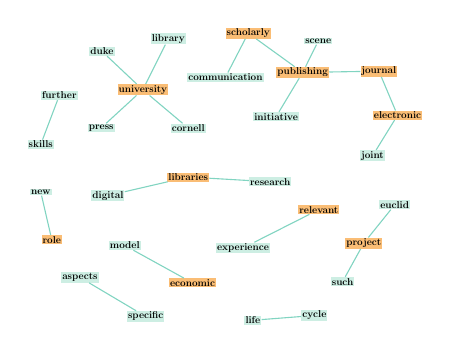
\begin{tikzpicture}[thin,
                              auto,
                              scale=.25,
                              align=center,
                              node distance=2cm,
                              every node/.style={font=\small, transform shape},
                              main node/.style={text centered,
                                                thick,
                                                fill=JungleGreen!20,
                                                inner sep=1.5pt,
                                                font=\Large\bfseries}]
            % connected component
            \node[main node, fill=BurntOrange!50] (university) {university};
            \node[main node] (duke) [above left=of university.north] {duke};
            \node[main node] (library) [above=of university.north east] {library};
            \node[main node] (press) [below left=of university.south] {press};
            \node[main node] (cornell) [below right=of university.south] {cornell};

            \path[JungleGreen!50] (university) edge (library);
            \path[JungleGreen!50] (university) edge (duke);
            \path[JungleGreen!50] (university) edge (press);
            \path[JungleGreen!50] (university) edge (cornell);

            % connected component
            \node[main node] (further) [left=of university.south west] {further};
            \node[main node] (skills) [below=of further.south west] {skills};

            \path[JungleGreen!50] (skills) edge (further);

            % connected component
            \node[main node, fill=BurntOrange!50] (scholarly) [right=of library.north east] {scholarly};
            \node[main node] (communication) [below=of scholarly.west] {communication};
            \node[main node, fill=BurntOrange!50] (publishing) [below right=of scholarly.south] {publishing};
            \node[main node] (scene) [above right=of publishing.west] {scene};
            \node[main node] (initiative) [below=of publishing.west] {initiative};
            \node[main node, fill=BurntOrange!50] (journal) [below right=of scene.north east] {journal};
            \node[main node, fill=BurntOrange!50] (electronic) [below=of journal.east] {electronic};
            \node[main node] (joint) [below=of electronic.north west] {joint};

            \path[JungleGreen!50] (communication) edge (scholarly);
            \path[JungleGreen!50] (publishing) edge (scholarly);
            \path[JungleGreen!50] (publishing) edge (scene);
            \path[JungleGreen!50] (publishing) edge (journal);
            \path[JungleGreen!50] (publishing) edge (initiative);
            \path[JungleGreen!50] (journal) edge (electronic);
            \path[JungleGreen!50] (joint) edge (electronic);

            % connected component
            \node[main node] (new) [below=of skills.south] {new};
            \node[main node, fill=BurntOrange!50] (role) [below=of new.south east] {role};

            \path[JungleGreen!50] (new) edge (role);

            % connected component
            \node[main node] (digital) [right=of new.south east] {digital};
            \node[main node, fill=BurntOrange!50] (libraries) [below =of cornell.south] {libraries};
            \node[main node] (research) [right =of libraries.south east] {research};

            \path[JungleGreen!50] (digital) edge (libraries);
            \path[JungleGreen!50] (libraries) edge (research);

            % connected component
            \node[main node, fill=BurntOrange!50] (relevant) [below right=of research.north] {relevant};
            \node[main node] (experience) [below left=of relevant.south west] {experience};

            \path[JungleGreen!50] (relevant) edge (experience);

            % connected component
            \node[main node] (model) [below=of digital.south east] {model};
            \node[main node, fill=BurntOrange!50] (economic) [below right=of model.south east] {economic};

            \path[JungleGreen!50] (model) edge (economic);

            % connected component
            \node[main node] (specific) [below left=of economic.center] {specific};
            \node[main node] (aspects) [above left=of specific.north west] {aspects};

            \path[JungleGreen!50] (specific) edge (aspects);

            % connected component
            \node[main node] (life) [below right=of economic.south east] {life};
            \node[main node] (cycle) [right=of life.north east] {cycle};

            \path[JungleGreen!50] (life) edge (cycle);

            % connected component
            \node[main node] (euclid) [right=of relevant.north east] {euclid};
            \node[main node, fill=BurntOrange!50] (project) [below left=of euclid.south east] {project};
            \node[main node] (such) [below left=of project.south east] {such};

            \path[JungleGreen!50] (euclid) edge (project);
            \path[JungleGreen!50] (project) edge (such);
          \end{tikzpicture}
        }{
          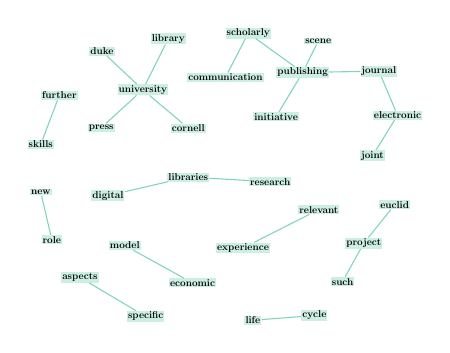
\begin{tikzpicture}[thin,
                              auto,
                              scale=.25,
                              align=center,
                              node distance=2cm,
                              every node/.style={font=\small, transform shape},
                              main node/.style={text centered,
                                                thick,
                                                fill=JungleGreen!20,
                                                inner sep=1.5pt,
                                                font=\Large\bfseries}]
            % connected component
            \node[main node] (university) {university};
            \node[main node] (duke) [above left=of university.north] {duke};
            \node[main node] (library) [above=of university.north east] {library};
            \node[main node] (press) [below left=of university.south] {press};
            \node[main node] (cornell) [below right=of university.south] {cornell};

            \path[JungleGreen!50] (university) edge (library);
            \path[JungleGreen!50] (university) edge (duke);
            \path[JungleGreen!50] (university) edge (press);
            \path[JungleGreen!50] (university) edge (cornell);

            % connected component
            \node[main node] (further) [left=of university.south west] {further};
            \node[main node] (skills) [below=of further.south west] {skills};

            \path[JungleGreen!50] (skills) edge (further);

            % connected component
            \node[main node] (scholarly) [right=of library.north east] {scholarly};
            \node[main node] (communication) [below=of scholarly.west] {communication};
            \node[main node] (publishing) [below right=of scholarly.south] {publishing};
            \node[main node] (scene) [above right=of publishing.west] {scene};
            \node[main node] (initiative) [below=of publishing.west] {initiative};
            \node[main node] (journal) [below right=of scene.north east] {journal};
            \node[main node] (electronic) [below=of journal.east] {electronic};
            \node[main node] (joint) [below=of electronic.north west] {joint};

            \path[JungleGreen!50] (communication) edge (scholarly);
            \path[JungleGreen!50] (publishing) edge (scholarly);
            \path[JungleGreen!50] (publishing) edge (scene);
            \path[JungleGreen!50] (publishing) edge (journal);
            \path[JungleGreen!50] (publishing) edge (initiative);
            \path[JungleGreen!50] (journal) edge (electronic);
            \path[JungleGreen!50] (joint) edge (electronic);

            % connected component
            \node[main node] (new) [below=of skills.south] {new};
            \node[main node] (role) [below=of new.south east] {role};

            \path[JungleGreen!50] (new) edge (role);

            % connected component
            \node[main node] (digital) [right=of new.south east] {digital};
            \node[main node] (libraries) [below =of cornell.south] {libraries};
            \node[main node] (research) [right =of libraries.south east] {research};

            \path[JungleGreen!50] (digital) edge (libraries);
            \path[JungleGreen!50] (libraries) edge (research);

            % connected component
            \node[main node] (relevant) [below right=of research.north] {relevant};
            \node[main node] (experience) [below left=of relevant.south west] {experience};

            \path[JungleGreen!50] (relevant) edge (experience);

            % connected component
            \node[main node] (model) [below=of digital.south east] {model};
            \node[main node] (economic) [below right=of model.south east] {economic};

            \path[JungleGreen!50] (model) edge (economic);

            % connected component
            \node[main node] (specific) [below left=of economic.center] {specific};
            \node[main node] (aspects) [above left=of specific.north west] {aspects};

            \path[JungleGreen!50] (specific) edge (aspects);

            % connected component
            \node[main node] (life) [below right=of economic.south east] {life};
            \node[main node] (cycle) [right=of life.north east] {cycle};

            \path[JungleGreen!50] (life) edge (cycle);

            % connected component
            \node[main node] (euclid) [right=of relevant.north east] {euclid};
            \node[main node] (project) [below left=of euclid.south east] {project};
            \node[main node] (such) [below left=of project.south east] {such};

            \path[JungleGreen!50] (euclid) edge (project);
            \path[JungleGreen!50] (project) edge (such);
          \end{tikzpicture}
        }
      \end{column}
      \begin{column}{.4\textwidth}
        \alt<5->{
          \resizebox{\linewidth}{!}{
            \begin{tabular}{l}
              Extracted Keyphrases\\
              \midrule
              electronic journal publishing\\
              \cellcolor{pink}scholarly publishing\\
              libraries\\
              university\\
              project\\
              economic\\
              relevant\\
              role
            \end{tabular}
          }
        }{
          \uncover<4>{
            \resizebox{\linewidth}{!}{
              \begin{tabular}{l}
                Extracted Keyphrases\\
                \midrule
                electronic journal publishing\\
                scholarly publishing\\
                libraries\\
                university\\
                project\\
                economic\\
                relevant\\
                role
              \end{tabular}
            }
          }
        }
      \end{column}
    \end{columns}

    \begin{block}<6->{Drawbacks}
      \begin{itemize}
        \item{Word nodes}
        \item{Co-occurence window}
        \item{Several nodes for one topic}
      \end{itemize}
    \end{block}
  \end{frame}


  \section{Co-ranking for Keyphrase Annotation}
\label{sec:topicrankpp}

  This section presents TopicCoRank\footnote{TopicCoRank will soon be publicly available on GitHub.}, our keyphrase annotation method.
  We first describe TopicRank~\cite{bougouin2013topicrank}, the 
  graph-based ranking approach to keyphrase extraction on which we build.
  We then present our unified graph model, and the co-ranking
  strategy we propose for performing both keyphrase extraction and assignment.
  
  \subsection{TopicRank}
  \label{subsec:topicrank}
    TopicRank is an unsupervised graph-based method that topically clusters the
    keyphrase candidates of a document, ranks the topics (topical clusters) and extracts the
    most representative keyphrase for each of the $N$ most important topics. It
    relies on four main steps: topical clustering, graph construction,
    graph-based topic ranking and extraction of the most representative keyphrase
    per topic.
    
    Sequences of adjacent words restricted to nouns and adjectives (\texttt{/(N|A)+/}) are 
    considered as keyphrase candidates.
    In TopicRank, similar keyphrase candidates are clustered into topics based
    on the words they share.
    \newcite{bougouin2013topicrank} use a Hierarchical
    Agglomerative Clustering (HAC) with a stem overlap similarity (see equation~\ref{math:jaccard}) and an average linkage: at
    the beginning, each keyphrase candidate is a single cluster, then candidates
    sharing an average of $\unitfrac{1}{4}$ stemmed words with the candidates of
    another cluster are iteratively added to the latter.
    \begin{align}
      \text{sim}(v_i, v_j) &= \frac{|\text{stems}(v_i) \cap \text{stems}(v_j)|}{|\text{stems}(v_i) \cup \text{stems}(v_j)|} \label{math:jaccard}
    \end{align}
    
    A complete graph is built, in which nodes are topics and edges are weighted according to the strength of the semantic
    relation between the connected topics. The closer two topics occur in the
    document, the stronger is their semantic relation.
    
    The importance ranking of the topics is performed with TextRank, modified to exploit edge
    weights $w$~\cite{wan2008expandrank} (see equation~\ref{math:singlerank}).
    \begin{align}
      S(v_i) = (1 - \lambda) + \lambda \sum_{v_j \in E(v_i)}{\frac{w_{ij}S(v_j)}{\mathlarger\sum_{v_k \in E(v_j)}{w_{jk}}}}\label{math:singlerank}
    \end{align}
      
    The keyphrase extraction is performed on the $N$  most important topics. To
    avoid topic redundancy, only one
    keyphrase per topic is extracted.
    Following previous observations~\cite{witten1999kea},
    the first occurring keyphrase candidate is chosen.

  \subsection{Graph construction for co-ranking}
  \label{subsec:graph_construction}
    TopicCoRank operates over a unified graph that connects two graphs
    representing the controlled keyphrases, the document topics and
    the relations between them. Controlled keyphrases are keyphrases
    that were manually assigned to training documents. We consider the 
    controlled keyphrases
    to be our controlled vocabulary for the keyphrase assignment.
    As controlled keyphrases are presumably non-redundant, we do not 
    group them by topics as we do for keyphrase candidates.
    
    Let
    $G = (V, E=E_{\textnormal{\textit{in}}} \cup E_{\textnormal{\textit{out}}})$
    denote the unified graph. Controlled keyphrases and topics are vertices $V$
    connected to their fellows by edges $E_\textnormal{\textit{in}}$ and
    connected to the other vertices by edges $E_\textnormal{\textit{out}}$ (see
    Figure~\ref{fig:topicrankpp_graph})\footnote{$E_\textnormal{\textit{in}} \subset V \times V$, $E_\textnormal{\textit{out}} \subset V \times V$, and $E_\textnormal{\textit{in}} \cup E_\textnormal{\textit{out}} = \emptyset$.}.
    
    \begin{figure*}
      \newcommand{\xslant}{0.25}
      \newcommand{\yslant}{0}

      \centering
      \begin{tikzpicture}[transform shape, scale=.667]
        % frame
        \node [draw,
               rectangle,
               minimum width=.9\linewidth,
               minimum height=7em,
               xslant=\xslant,
               yslant=\yslant] (domain_graph) {};
        \node [above=of domain_graph,
               xshift=.45\linewidth,
               yshift=7em,
               anchor=south east] (domain_graph_label) {controlled keyphrases};

        \node [draw,
               circle,
               above=of domain_graph,
               xshift=.3\linewidth,
               yshift=4em] (domain_node1) {$v_1$};
        \node [draw,
               circle,
               above=of domain_graph,
               xshift=-.3\linewidth,
               yshift=4em] (domain_node2) {$v_2$};
        \node [draw,
               circle,
               above=of domain_graph,
               yshift=4em] (domain_node3) {$v_3$};
        \node [draw,
               circle,
               above=of domain_graph,
               xshift=.15\linewidth,
               yshift=.75em] (domain_node4) {$v_4$};
        \node [draw,
               circle,
               above=of domain_graph,
               xshift=-.15\linewidth,
               yshift=.75em] (domain_node5) {$v_5$};

        \draw (domain_node1) -- (domain_node3);
        \draw (domain_node2) -- (domain_node3);
        \draw (domain_node2) -- (domain_node4);
        \draw (domain_node4) -- (domain_node5);
        \draw (domain_node4) -- (domain_node3);

        % document
        \node [draw,
               rectangle,
               minimum width=.9\linewidth,
               minimum height=7em,
               xslant=\xslant,
               yslant=\yslant,
               above=of domain_graph,
               xshift=-2em] (document_graph) {};
        \node [below=of document_graph,
               xshift=-.45\linewidth,
               yshift=-7em,
               anchor=north west] (document_graph_label) {document topics};

        \node [draw,
               circle,
               below=of document_graph,
               xshift=.3\linewidth,
               yshift=-4em] (document_node1) {$v_6$};
        \node [draw,
               circle,
               below=of document_graph,
               xshift=-.3\linewidth,
               yshift=-4em] (document_node2) {$v_7$};
        \node [draw,
               circle,
               below=of document_graph,
               yshift=-4em] (document_node3) {$v_8$};
        \node [draw,
               circle,
               below=of document_graph,
               xshift=.15\linewidth,
               yshift=-.75em] (document_node4) {$v_9$};

        \draw (document_node2) -- (document_node3);
        \draw (document_node3) -- (document_node1);
        \draw (document_node1) -- (document_node4);
        \draw (document_node3) -- (document_node4);

        % extra link
        \draw [dashed] (document_node2) -- (domain_node2);
        \draw [dashed] (document_node3) -- (domain_node3);
        \draw [dashed] (document_node4) -- (domain_node1);
        \draw [dashed] (document_node3) -- (domain_node4);

        % legend
        \node [right=of document_graph, xshift=2em, yshift=-8em] (legend_title) {\underline{Legend:}};
        \node [below=of legend_title, xshift=-1em, yshift=2em] (begin_inner) {};
        \node [right=of begin_inner] (end_inner) {: $E_\textnormal{\textit{in}}$};
        \node [below=of begin_inner, yshift=1.5em] (begin_outer) {};
        \node [right=of begin_outer] (end_outer) {: $E_\textnormal{\textit{out}}$};

        \draw (legend_title.north  -| end_outer.east) rectangle (end_outer.south -| legend_title.west);

        \draw (begin_inner) -- (end_inner);
        \draw [dashed] (begin_outer) -- (end_outer);
      \end{tikzpicture}
      \caption{Example of a unified graph constructed by TopicCoRank and its two
               kinds of edges
               \label{fig:topicrankpp_graph}}
    \end{figure*}

    To unify the two graphs, we consider the controlled keyphrases as a category map and connect the document to its potential categories. We create an edge
    $\langle{}v_i, v_j\rangle{} \in E_{\textnormal{\textit{out}}}$ to connect a controlled
    keyphrase $v_i$ and a topic $v_j$ if the controlled keyphrase is a
    member of the topic, i.e., a keyphrase candidate in the topic.
    To accept flexions, such as plural flexions, we perform the comparison with
    stems.
    We create an edge $\langle{}v_i, v_j\rangle{} \in E_\textnormal{\textit{in}}$ between two controlled
    keyphrases or two topics $v_i$ and $v_j$ when they co-occur, respectively, as keyphrases of
    a training document or within a sentence of the
    document. Each edge $\langle{}v_i, v_j\rangle{} \in E_{\textnormal{\textit{in}}}$ is weighted by
    the normalized number of co-occurrences $w_{ij}$ of the controlled
    keyphrases or the topics $v_i$ and $v_j$ within the keyphrase sets of each training document or the document, respectively. The weighting scheme of edges
    $E_\textnormal{\textit{in}}$ is equivalent for both controlled keyphrases and
    topics. This equivalence is essential to properly co-rank controlled keyphrases
    and topics and, therefore, ensure that not only controlled keyphrases occurring in the document can be assigned.

  \subsection{Graph-based co-ranking}
  \label{subsec:graph_based_co_ranking}
    TopicCoRank gives an importance score $S(v_i)$ to every vertex
    $v_i$ using graph co-ranking (see equation~\ref{math:topiccorank}).
    Graph co-ranking has been applied with success to many NLP tasks 
    such as text summarization~\cite{wan2011corankingsummarization}, 
    tweet recommendation~\cite{yan2012corankingtweetrecommendation} or 
    opinion mining~\cite{liu2014corankingopinionmining}.
    
    The
    graph co-ranking simulates the ``voting concept'' based on inner and outer
    recommendations. The inner recommendation $R_\textnormal{\textit{in}}$ of a
    node comes from nodes of the same graph (see equation~\ref{math:rin}):
    \begin{itemize}
      \item{a controlled keyphrase is important if it is strongly connected to other
            controlled keyphrases;}
      \item{a topic is important if it is strongly connected to other topics.}
    \end{itemize}
    The outer recommendation $R_\textnormal{\textit{out}}$ of a node comes from nodes
    of the other graph (see equation~\ref{math:rout}):
    \begin{itemize}
      \item{a controlled keyphrase is more important in the context of the document if it
            is connected to one of its important topics;}
      \item{a topic is more important if it is connected to important controlled keyphrases.}
    \end{itemize}
    \begin{align}
      S(v_i) &= (1 - \lambda)\ R_{out}(v_i) + \lambda\ R_{in}(v_i)\label{math:topiccorank}\\
      R_{in}(v_i) &= \sum_{v_j \in E_{\text{in}}(v_i)}{\frac{w_{ij} S(v_j)}{\mathlarger\sum_{v_k \in E_{\text{in}}(v_j)}{{w_{jk}}}}}\label{math:rin}\\
      R_{out}(v_i) &= \sum_{v_j \in E_{\text{out}}(v_i)}{\frac{S(v_j)}{|E_{\text{\textit{out}}}(v_j)|}}\label{math:rout}
    \end{align}
    $\lambda$ is a parameter that controls the influence of the inner recommendation
    over the outer recommendation ($0 \leq \lambda \leq 1$). A higher $\lambda$
    gives more influence to the inner recommendation and a lower $\lambda$ gives
    more influence to the outer recommendation. By default, we set $\lambda$ to $0.5$
    to give the same impact to both recommendations.

    \begin{table*}
      \centering
      %\resizebox{.8\linewidth}{!}{
          \begin{tabular}{l|cccc|cc}
            \toprule
            \multirow{2}{*}{\textbf{Corpus}} & \multicolumn{4}{c|}{\textbf{Documents}} & \multicolumn{2}{c}{\textbf{Keyphrases}}\\
            \cline{2-7}
            & Type & Language & Number & Tokens average & Average & Missing\\
            \hline
            Linguistics & & & & & &\\
            $\drsh$~train & Abstracts & French & 515 & $~~$161 & $~~$8.6 & 60.6\%\\
            $\drsh$~test & Abstracts & French & 200 & $~~$147 & $~~$8.9 & 62.8\% \\
            \hline
            Archaeology & & & & & &\\
            $\drsh$~train & Abstracts & French & 518 & $~~$221 & 16.9 & 37.0\%\\
            $\drsh$~test & Abstracts & French & 200 & $~~$214 & 15.6 & 37.4\%\\
            \hline
            DUC & News & English & 308 & $~~$901 & $~~$8.1 & $~~$3.5\%\\
            \hline
            SemEval & & & & & &\\
            $\drsh$~train & Papers & English & 144 & 5135 & 15.4 & 13.5\%\\
            $\drsh$~test & Papers & English & 100 & 5178 & 14.7 & 22.1\%\\
            \bottomrule
          \end{tabular}
      %}
      \caption{Dataset statistics. ``Missing'' represents the percentage of keyphrases
               that cannot be retrieved within the documents.
               \label{tab:corpus_statistics}}
    \end{table*}

  \subsection{Keyphrase annotation}
  \label{subsec:keyphrase_assignment_and_extraction}
    To both assign and extract keyphrases, we sort the controlled
    keyphrases and the topics based on their importance score $S$. The $N$-best ranking ones are
    considered as the keyphrases of the document regardless of their nature (topic keyphrase or controlled keyphrase).

    We assign controlled keyphrases over one condition. A controlled keyphrase can
    be assigned to a document if it is directly or transitively connected to a
    topic of the document. Indeed, if the ranking of a controlled keyphrase has not been
    affected by topics of the document nor controlled keyphrases connected to topics,
    its importance score is not related to the content of the document and we do not
    want to assign them.

    We extract keyphrases from the topics using the former TopicRank strategy.
    Only one keyphrase is extracted per topic: the
    candidate that occurs first within the document.

  \section{Experimental Settings}
\label{sec:experimental_settings}
  \subsection{Datasets}
  \label{subsec:datasets}
    We run experiments over three datasets: Inspec, SemEval and Inist (ling.),
    which differ in terms of language, nature and size. The following is the
    description of each dataset.

    \paragraph{Inspec~\textnormal{\cite{hulth2003keywordextraction}}} contains
    2000 English abstracts of journal papers collected from the Inspec database.
    The abstracts cover two fields of Computer Science: Computers and Control;
    Information Technology. Inspec is divided into three disjoint sets: a trial
    set containing 500 abstract, a training set containing 1000 abstracts and a
    test set containing 500 abstracts. \TODO{explain keyphrases set and chose
    which one to use}

    \paragraph{SemEval~\textnormal{\cite{kim2010semeval}}} contains 244 English
    scientific papers collected from the ACM Digital Libraries (conference and
    workshop papers). The papers represent four areas of Computer Science:
    Distributed Systems; Information Search and Retrieval; Distributed
    Artificial Intelligence -- Multiagent Systems; Social and Behavioral
    Sciences -- Economics. SemEval is divided into two disjoint sets: a training
    set containing 144 documents and a test set containing 100 documents. The
    associated keyphrases are provided by both authors and readers.

    \paragraph{Inist (ling.)} \TODO{uncertain yet}

    \paragraph{}
    Table~\ref{tab:corpus_statistics} shows factual information about each
    datasets. By looking at these, one can understand the importance of methods
    like ours. Indeed, ranging from \TODO{0.0\%} to \TODO{100\%}, the percentage
    of keyphrases impossible to extract from the documents is part of the
    keyphrases our method is able to find.

  \subsection{Preprocessing}
  \label{subsec:preprocessing}
    We apply the following preprocessing steps to every document of the
    datasets: sentence segmentation, word tokenization and Part-of-Speech (POS)
    tagging. We perform sentence segmentation with the PunktSentenceTokenizer
    provided by the Python Natural Language ToolKit~\cite[NLTK]{bird2009nltk}.
    We tokenize the sentence into words using the NLTK TreebankWordTokenizer for
    English and the Bonsai word tokenizer\footnote{The Bonsai word tokenizer is
    a tool provided with the Bonsai PCFG-LA parser:
    \url{http://alpage.inria.fr/statgram/frdep/fr_stat_dep_parsing.html}.} for
    French. Finally, we use the Stanford POS
    tagger~\cite{toutanova2003stanfordpostagger} for English POS tagging and
    MElt~\cite{denis2009melt} for French POS tagging.

  \subsection{Baselines}
  \label{subsec:baselines}
    We compare TopicRank++ with TopicRank and TopicRank++ when only domain
    keyphrases are extracted (TopicRank++$_\textnormal{\textit{dom.}}$), when
    only document keyphrases are extracted
    (TopicRank++$_\textnormal{\textit{doc.}}$) and when the co-ranking is
    performed with candidate keyphrases instead of topics
    (TopicRank++$_\textnormal{\textit{cdt}}$).

  \subsection{Evaluation measures}
  \label{subsec:evaluation_measures}
    To evaluate the performance of the keyphrase extraction methods, we use the
    common measures of precision (P), recall (R) and f-score (F). We cut-off the
    extracted keyphrases at the 10 best ranking ones.


  \section{Evaluation}
  \begin{frame}{Evaluation}
    \framesubtitle{Datasets}

    \begin{itemize}
      \item{Inspec contains 500 abstracts of journal papers ({\small\textsc{En}})}
      \begin{itemize}
        \setbeamertemplate{itemize items}[triangle]
        \item{9.8 keyphrases/document}
        \item{21.8\% of missing keyphrases}
      \end{itemize}
    \item{SemEval contains 100 scientific papers ({\small\textsc{En}})}
      \begin{itemize}
        \setbeamertemplate{itemize items}[triangle]
        \item{14.7 keyphrases/document}
        \item{19.3\% of missing keyphrases}
      \end{itemize}
      \item{WikiNews contains 100 news articles ({\small\textsc{Fr}})}
      \begin{itemize}
        \setbeamertemplate{itemize items}[triangle]
        \item{9.6 keyphrases/document}
        \item{4.4\% of missing keyphrases}
      \end{itemize}
      \item{DEFT contains 93 scientific papers ({\small\textsc{Fr}})}
      \begin{itemize}
        \setbeamertemplate{itemize items}[triangle]
        \item{5.2 keyphrases/document}
        \item{18.2\% of missing keyphrases}
      \end{itemize}
    \end{itemize}
  \end{frame}

  \begin{frame}{Evaluation}
    \framesubtitle{Evaluation measures}

    \begin{itemize}
      \item{Cut-off at 10 keyphrases}
      \item{F-score $\Rightarrow$ compromise between precision and recall}
    \end{itemize}

    \begin{center}
      $\text{f-score} = (1 + \beta^2) \times \frac{\text{precision} \times \text{recall}}{(\beta^2 \times precision) + recall}$,
      $\beta = 1$
    \end{center}
  \end{frame}

  \begin{frame}{Evaluation}
    \framesubtitle{Baselines}

    \begin{itemize}
      \item{TF-IDF weighting}
      \begin{itemize}
        \setbeamertemplate{itemize items}[triangle]
        \item{Best keyphrases contain words with hight TF-IDF}
      \end{itemize}
      \item{TextRank}
      \begin{itemize}
        \setbeamertemplate{itemize items}[triangle]
        \item{Word co-occurrence graph with a window of 2}
        \item{PageRank scoring/ranking}
        \item{Keyphrase generation based on keywords}
      \end{itemize}
      \item{SingleRank}
      \begin{itemize}
        \setbeamertemplate{itemize items}[triangle]
        \item{Word co-occurrence graph with a window of 10}
        \item{PageRank scoring/ranking}
        \item{Candidate keyphrases scored/ranked by the sum of their words' PageRank score}
      \end{itemize}
    \end{itemize}

    Redundant keyphrases are removed from the output.
  \end{frame}

  \begin{frame}{Evaluation}
    \framesubtitle{Main results}
    
    \begin{center}
      \begin{tabular}{rcccc}
        \toprule
        Methods & Inspec & SemEval & WikiNews & DEFT\\
        \midrule
        TF-IDF & 33.4 & 10.5 & 34.3 & 13.2\\
        TextRank & 12.7 & $~~$5.6 & $~~$8.6 & $~~$5.7\\
        SingleRank & \cellcolor{pink}{35.2} & $~~$3.7 & 19.7 & $~~$5.9\\
        TopicRank & 27.9 & \cellcolor{pink}{12.1} & \cellcolor{pink}{35.6} & \cellcolor{pink}{15.1}\\
        \bottomrule
      \end{tabular}
    \end{center}
  \end{frame}

  \begin{frame}{Evaluation}
    \framesubtitle{Contributions evaluation}
    
    \begin{center}
      \begin{tabular}{rcccc}
        \toprule
        Methods & Inspec & SemEval & WikiNews & DEFT\\
        \midrule
        SingleRank & 35.2 & $~~$3.7 & 19.7 & $~~$5.9\\
        +phrases & 22.1 & $~~$8.0 & 28.9 & 13.5\\
        +topics & 26.8 & 11.9 & 31.4 & 14.8\\
        +complete &  \cellcolor{pink}{35.5} & $~~$4.4 & 20.3 & $~~$5.8\\
        TopicRank & 27.9 & \cellcolor{pink}{12.1} & \cellcolor{pink}{35.6} & \cellcolor{pink}{15.1}\\
        \bottomrule
      \end{tabular}
    \end{center}
  \end{frame}

  \begin{frame}{Evaluation}
    \framesubtitle{Keyphrase selection evaluation}
    
    \begin{center}
      \resizebox{\linewidth}{!}{
        \begin{tabular}{rcccc}
          \toprule
          Keyphrase selection & Inspec & SemEval & WikiNews & DEFT\\
          \midrule
          \rowcolor{cyan!33} First position & 27.9 & 12.1 & 35.6 & 15.1\\
          Frequency & 26.8 & $~~$1.4 & 26.2 & $~~$2.5\\
          Centroid &  24.7 & $~~$1.5 & 28.5 & $~~$3.4\\
          \rowcolor{pink} Upper bound & 35.6 & 30.3 & 42.9 & 19.3\\
          \bottomrule
        \end{tabular}
      }
    \end{center}
  \end{frame}


  \section{Conclusion et perspectives}
\label{sec:conclusion_et_perspectives}
  Dans cet article, nous nous intéressons à la tâche d'extraction automatique de
  termes-clés dans les documents scientifiques et émettons l'hypothèse que sa
  difficulté est variable selon la discipline des documents traités. Pour
  vérifier cette hypothèse, nous disposons de notices bibliographiques réparties
  dans cinq disciplines (archéologie, linguistique, sciences de l'information,
  psychologie et chimie) auxquelles nous appliquons six systèmes d'extractions
  automatique de termes-clés différents. En comparant les termes-clés extraits
  par chaque système avec les termes-clés de référence assignés aux notices dans
  des conditions réels d'indexation, notre hypothèse se vérifie et nous
  observons l'échelle suivante (de la discipline la plus facile à la plus
  difficile)~:
  \begin{enumerate*}
    \item{Archéologie~;}
    \item{Linguistique~;}
    \item{Sciences de l'information~;}
    \item{Psychologie~;}
    \item{Chimie.}
  \end{enumerate*}

  À l'issue de nos expériences et de nos observations du contenu des notices,
  nous constatons deux facteurs ayant un impact sur la difficulté de la tâche
  d'extraction automatique de termes-clés. Tout d'abord, nous observons que
  l'organisation du résumé peut aider l'extraction de termes-clés. Un résumé
  riche en explications et en mises en relations des différents concepts est
  moins difficile à traiter qu'un résumé énumératif pauvre en explications.
  Ensuite, le vocabulaire utilisé dans une discipline peut influer sur la
  difficulté à extraire les termes-clés des documents de cette discipline. Si le
  vocabulaire spécifique contient des composés syntagmatiques dont certains
  éléments sont courants dans la discipline, alors il peut être plus difficile
  d'extraire les termes-clés des documents de cette discipline.

  Des deux facteurs identifiés émergent plusieurs perspectives de travaux
  futurs. Il peut être intéressant d'analyser le discours des documents afin de
  mesurer, en amont, le degré de difficulté de l'extraction de termes-clés. Avec
  une telle connaissance, nous pourrions proposer une méthode capable de
  s'adapter au degré de difficulté en ajustant automatiquement son paramètrage.
  Cependant, l'analyse que nous proposons dans cet article se fonde uniquement
  sur le contenu de notices appartenant à cinq disciplines. Il serait pertinent
  d'étendre cette analyse au contenu intégral des documents scientifiques, ainsi
  que d'élargir le panel de disciplines utilisées dans ce travail, afin
  d'établir des catégories de discplines plus ou moins difficiles à traiter
  (p.~ex. la chimie fait partie des disciplines expérimentales, qui sont
  difficiles à traiter). Nous oberservons aussi que le vocabulaire utilisé dans
  une discipline, en particulier celui utilisé pour les termes-clés, peut rendre
  la tâche d'extraction automatique de termes-clés plus difficile. Il est donc
  important de bénéficier de resources telles que des thésaurus pour permettre à
  une méthode d'extraction de termes-clés de s'adapter au domaine. Pour
  TopicRank, par exemple, avoir connaissance de la terminologie utilisée dans
  une discipline peut améliorer le choix du terme-clé le plus représentatif d'un
  sujet. Enfin, il serait intéressant de penser la tâche d'extraction de
  termes-clés comme une tâche d'extraction d'information pour le remplissage
  d'un formulaire. En archéologie, par exemple, il pourrait s'agir d'extraire
  les informations géographiques (pays, régions, etc.), chronologiques (période,
  culture, etc.), ou encore environnementales (animaux, végétaux, etc.).



%  \section*{Acknowledgments}
%    The authors would like to thank the anonymous reviewers for their useful
%    advice and comments. This work was supported by the French National Research
%    Agency (TermITH project -- ANR-12-CORD-0029).

  \bibliographystyle{acl}
  \bibliography{../../biblio}
\end{document}
